\documentclass[runningheads,a4paper]{article}

\usepackage[utf8]{inputenc}

\setcounter{tocdepth}{3}

\usepackage[english]{babel} 
\usepackage{graphicx}
\usepackage{grffile}
\usepackage{float}
\usepackage{multicol}
\usepackage{url}

\usepackage{titling}
\usepackage[hidelinks]{hyperref}

%Margins
\usepackage[
margin=2cm,
includefoot
]{geometry}



%Headers and Footers
\usepackage{fancyhdr}
\pagestyle{fancy}
\fancyhead{}
\fancyfoot{}
\fancyfoot[R]{\thepage}
\renewcommand{\headrulewidth}{0pt}
\renewcommand{\footrulewidth}{0pt}
\setlength\parindent{24pt}
\begin{document}
	
	%Title Page
	\begin{titlepage}
		\begin{center}
			
\includegraphics[width=10cm]{img/UP.jpg}  \\
			[1cm]
			\line(1,0){300} \\
			[0.3cm]
			\textsc{\Large
				NavUP\\
				Architectural Requirements Specifications and Design \\
				\hfill \break 10 March 2017
				%University of Pretoria
			}\\
			[0.1cm]
			\line(1,0){300} \\
			[0.7cm]
			\textsc{\Large
				Team Scala
			} \\
			
			
			
		\end{center}
		
		\begin{center}
			\begin{multicols}{2}
				\textsc{\large\\
					Merissa Joubert \\ 
					15062440\\ 
				}
				
				\textsc{\large\\
					Joshua Cilliers \\
					14267196\\ 
				}
				
				\textsc{\large\\
					Gershom Maluleke \\
					13229908\\ 
				}
				
				\textsc{\large\\
					Peter Soroush\\
					13238958\\ 
				}
				
				\columnbreak
				
				\textsc{\large\\
					Avinash Singh\\
					14043778\\
				}
				
				\textsc{\large\\
					Nicolai Van Niekerk\\
					15025269\\
				}
				
				\textsc{\large\\
					Cameron Trivella\\
					14070970\\ 
				}
				
			\end{multicols}
			
			
			\textsc{	\\ \href{https://github.com/Rob0girl/Team-Scala.git}{GitHub}
				\url{https://github.com/Rob0girl/Team-Scala.git}}
			
		\end{center}
	\end{titlepage}
	%\maketitle
	
	\begingroup
	
	\tableofcontents
	\addcontentsline{toc}{section}{Table Of Contents}
	\endgroup
	\newpage
	
	\section{Introduction}
\subsection{Overview}
This document identifies the architectural design specifications that satisfy the functional requirements proposed in the System Requirements Specification. It addresses the needs of the various subsystems' non-functional requirements focusing on the quality attributes, architectural patterns as well as constraints and integration requirements of the NavUP system.\newline \newline 
The following modules' designs are included in this document:
\begin{itemize}
	\item Users
	\item GIS
	\item Notification
	\item Events
\end{itemize}
The document begins with an explanation on the chosen architectural pattern and how it will be used to modularize the NavUP system. It then outlines the architectural design of each module along with all relevant UML diagrams. Finally the chosen technologies are discussed as well as the deployment of the system. 

\subsection{Architectural Pattern}
The NavUP system will be designed using the Three-tier architecture in which the user-interface, process logic and data storage are developed and maintained as independent modules. This will allow any of the three tiers to be upgraded or replaced without affecting any of the other layers. \newline
The NavUP system will be divided into 3 tiers:
\begin{itemize}
	\item Presentation tier
	\item Application tier
	\item Data tier
\end{itemize} 

\subsubsection{Presentation tier}
This is the highest level of the NavUP application. It is the layer which users will interact with directly through the user-interface. The Presentation layer will reside on the mobile and web app and will display information pulled from the Application layer in a way that is simple and intuitive to the user of the application.

\subsubsection{Application tier}
This layer resides on the application server and controls the application's functionality through detailed processing. The results of this processing is passed back to the Presentation layer which will display it to the user.

\subsubsection{Data tier}
The Data layer includes all data persistence mechanisms and resides on the database server. The application server uses this layer to manage the stored data. It is crucial that there are no dependencies on the storage mechanisms to ensure that any updates or changes will not affect the application tier clients in any way.
\newpage
	

\section{User Module Sub-system}

\subsection{External Interfaces}
This section gives a detailed description of the system interfaces, hardware interfaces, software interfaces as well as communication interfaces.

	\subsubsection{System Interfaces}
		\begin{itemize}
			\item The user module will interface with any subsystem or module that wishes to access the data or functions.  
			
			\item 
		\end{itemize}
	\subsubsection{User Interfaces }
	\subsubsection{Hardware Interfaces }
	\subsubsection{Software Interfaces } %
	\subsubsection{Communication Interfaces } %
	
\subsection{Performance Requirements} %


\subsection{Design Constraints}



\subsection{Software System Attributes} %


\subsection{UML}
\subsubsection{Class Diagram}
The class diagram of the user sub-system makes use of the template method so that if need be one can easily construct different types of users with minimal code modifications.


\begin{figure}[H]
	\centering
	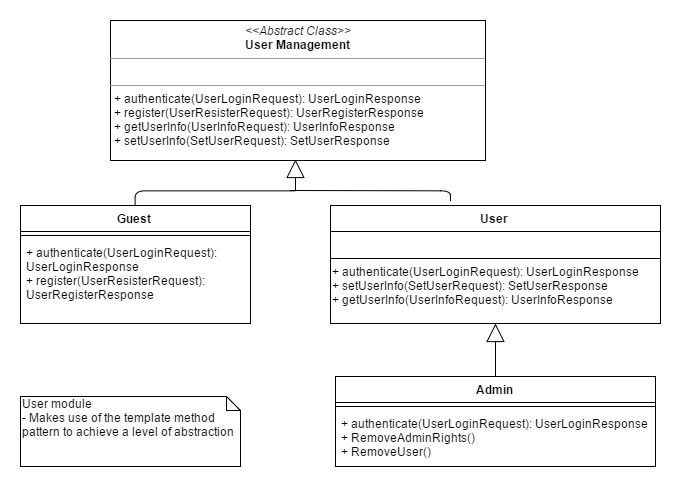
\includegraphics[width=0.7\textwidth]{user/img/UserClassDiagram.jpg}
	\caption{User Class Diagram}
\end{figure}



%\subsection{Deployment Diagram}
%
%\begin{figure}[H]
%%	\centering
%%	\includegraphics[width=\textwidth]{user/img/}
%%	\caption{}
%\end{figure}
%
%
\subsubsection{Activity Diagram}

\begin{figure}[H]
		\centering
		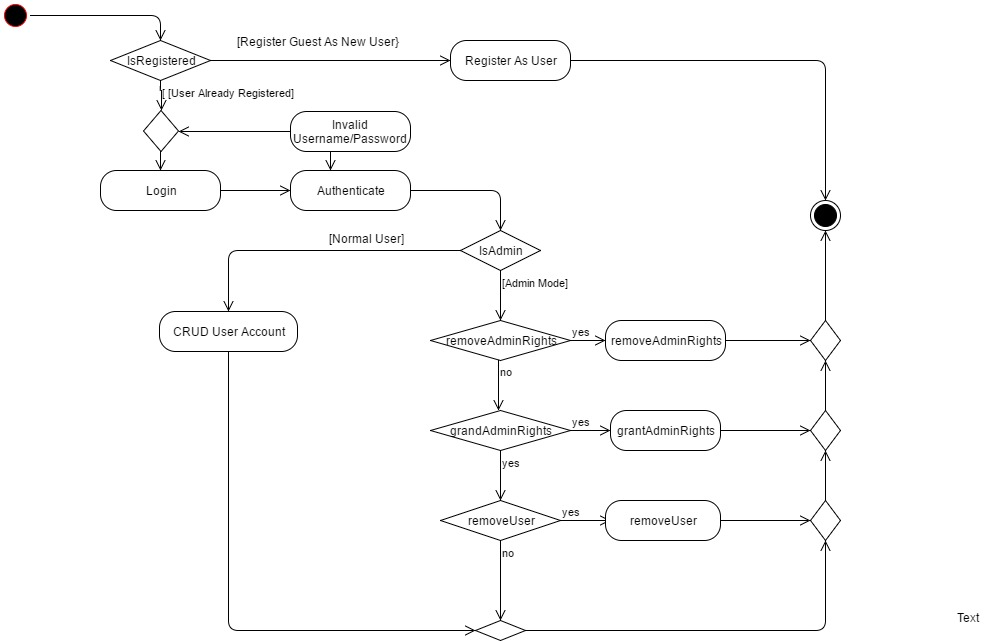
\includegraphics[width=\textwidth]{user/img/UserActivityDiagram.jpg}
		\caption{User Activity Diagram}
\end{figure}


\subsubsection{Sequence Diagram}

\begin{figure}[H]
		\centering
		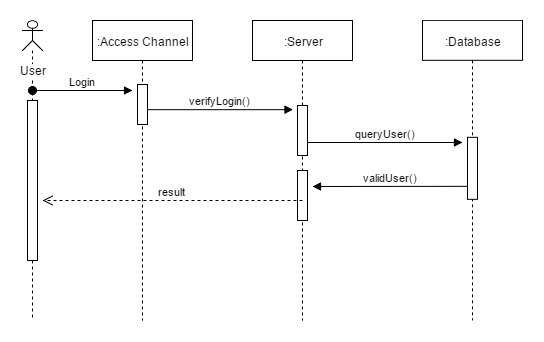
\includegraphics[width=0.7\textwidth]{user/img/UserSequence.jpg}
		\caption{User Login}
\end{figure}



\subsubsection{State Diagram}

\begin{figure}[H]
		\centering
		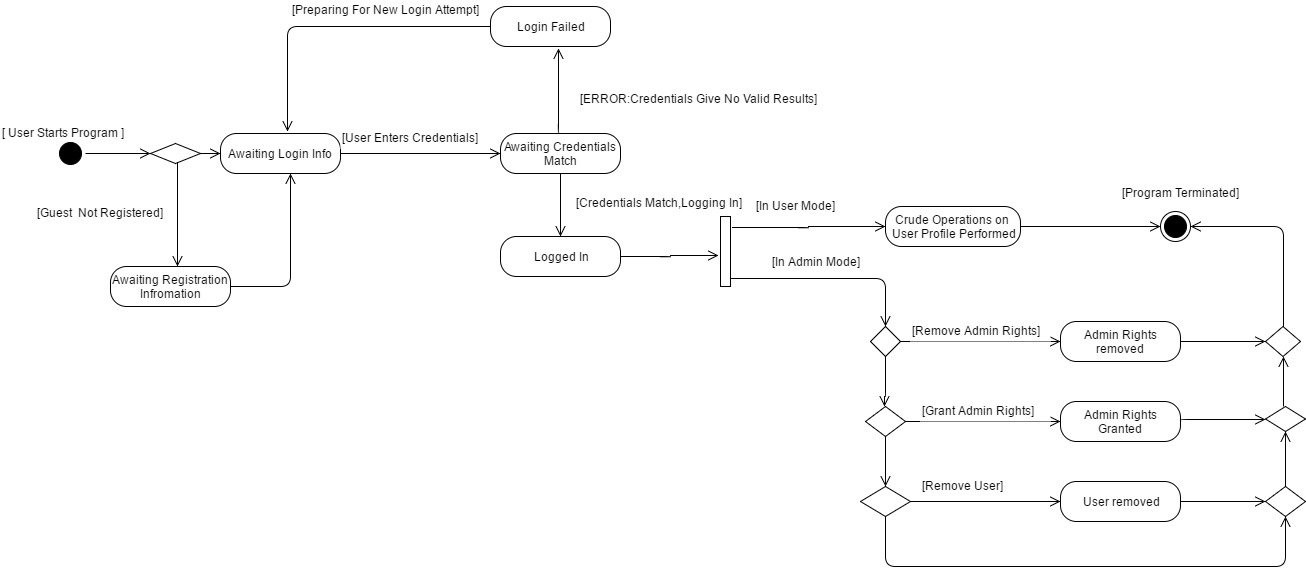
\includegraphics[width=\textwidth]{user/img/UserStateDiagram.jpg}
		\caption{User Login State Diagram}
\end{figure}




\subsubsection{Use Case Diagram}

\begin{figure}[H]
		\centering
		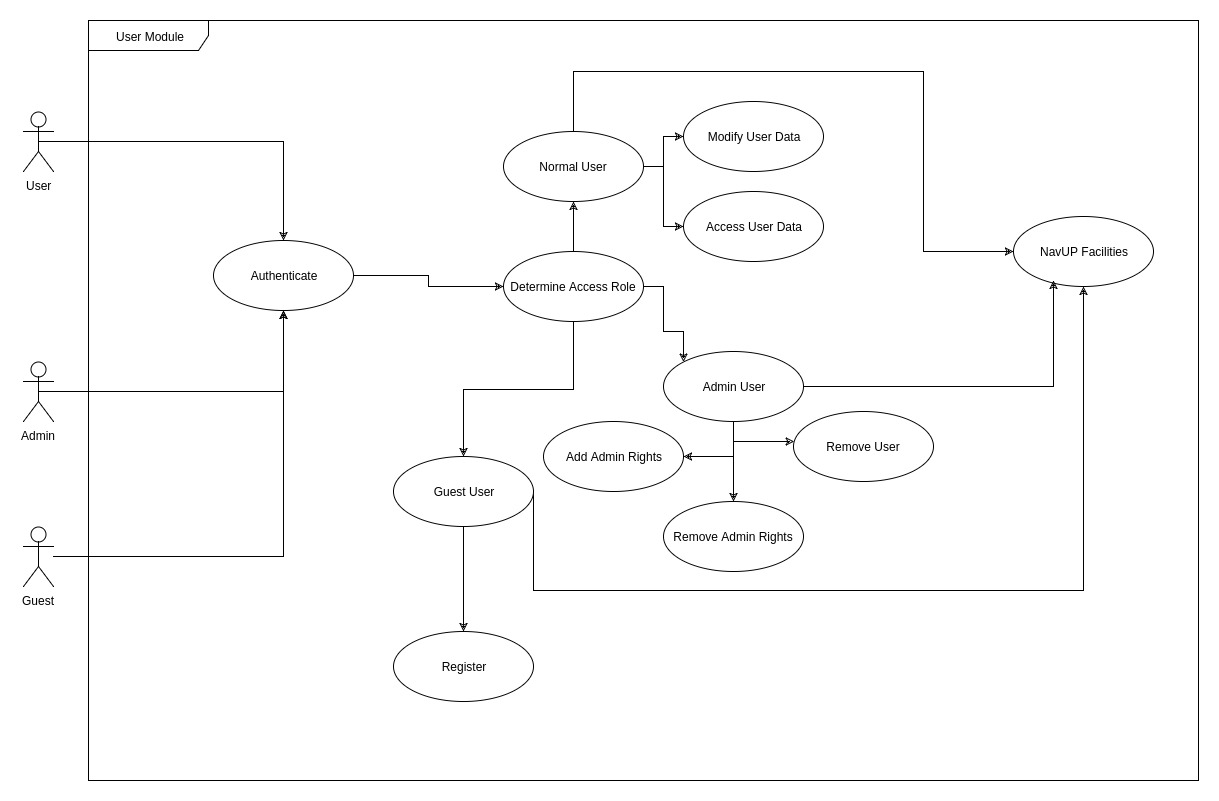
\includegraphics[width=0.7\textwidth]{user/img/UserUseCase.jpg}
		\caption{User Login with core functionality }
\end{figure}




	\pagebreak
	\section{GIS Module}

\subsection{Overview}
The GIS module provides services to gather, maintain, persist and provide information related to the world serviced by the system. It is about the creation and maintenance of a GIS Map of the
campus by using WiFi signal strengths and other available sources of GIS information. In addition it provides services to search for locations such as landmarks, buildings as well as venues such as offices, lecture halls and labs.

	\pagebreak
	\section{Event Module}
\subsection{Overview}
The Event module is responsible for the Event Management for example lectures, Programs, tests and events.
 
\subsection{External Interface Requirements}
This section gives a detailed description of the system interfaces, hardware interfaces, software interfaces as well as communication interfaces. 

	\subsubsection{System Interfaces}
		\begin{itemize}
			\item The user module will interface with any subsystem or module that wants to access Events.

			\item  The user module will interface with Notification to Notify User about Events
		
		\end{itemize}
	\subsubsection{User Interfaces }
	\begin{itemize} 

	\item User Interface is in Calander Form which Shows all the events in it.

 \end{itemize}
 
	\subsubsection{Hardware Interfaces }
	The Event Module does not have any explicit hardware interface

	\subsubsection{Software Interfaces } 
	The event module will communicate with the database in order to get the details of events, and also for saving and editing new Events etc. All the I/O interaction with the database.
	
	\subsubsection{Communication Interfaces } 
		\begin{itemize}
		\item The Event module will need to comunicate with Notification to notify Users.
		\item needs to comunicate with Users as only registered user can see Events.
		\end{itemize}

	
\subsection{Performance Requirements}
Event module should be able to perform under high CRUD operations,and have optimised methods to allow for faster execution and faster response times.


\subsection{Design Constraints}
\begin{itemize}

\item The speed at which NavUP can perform is constrained by the processing power and the  memory that is available on the device on which it runs.

\item This system’s ability to give updates and events to users through the Users module is constrained by the external management and maintenance which is performed by the administrator of the system.

\end{itemize}


\subsection{Software System Attributes} 
\subsubsection{Availability}
The Event module should always be active since the it has Time Countdown and also there is posibility od Changing and updating all the time. 
\subsubsection{Reliability}
The Event module should make use of queuing for CRUD database operations, which most databases have and should be reliable since the database should be ACID compliant.

\subsubsection{Security}
Data within the Event module should not have external classes accessing the information without being authenticated, only admins can modify Events and add them or remove it, so No Guest or Normal User must be able to access to editing functionalities, also not registered User cannot see Events.

\subsubsection{Auditability}
As Admin,Normal and Guest Users have different Authorities to View and Modify Events, so user must be Logged on the Back-end Server before Getting to Events section

 
\subsection{UML}
\subsubsection{Class Diagram}
The class diagram of the Events sub-system makes use of the template method design pattern so that if need be one can easily construct different types of Event with minimal code modifications.

\begin{figure}[H]
	\centering
	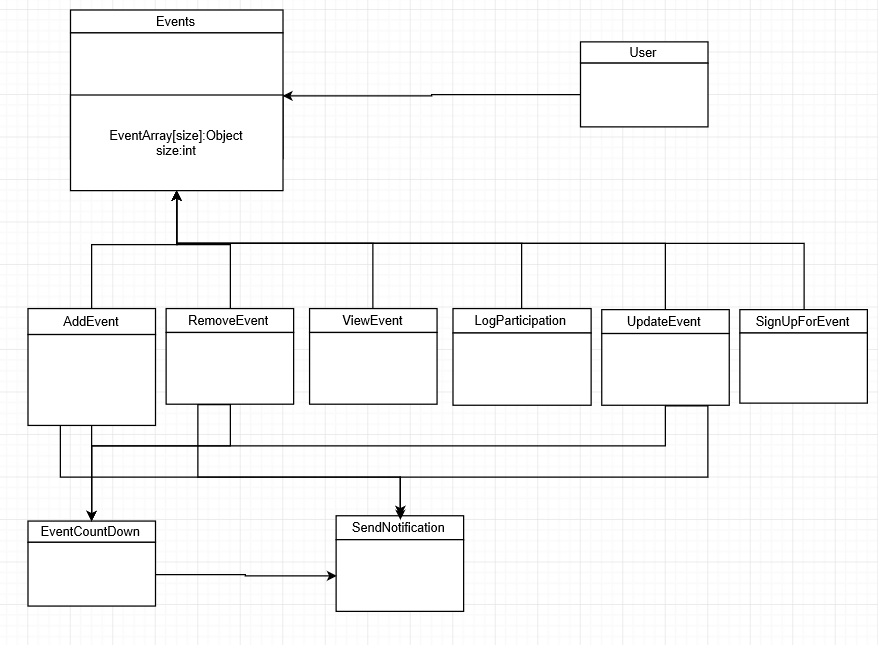
\includegraphics[width=0.7\textwidth]{event/ClassDiagrams(NoMethods).PNG}
	\caption{Event Class Diagram}
\end{figure}



\pagebreak
\subsubsection{Activity Diagram}
This diagram models work-flow activities of what users can do in the Event module.

\begin{figure}[H]
		\centering
		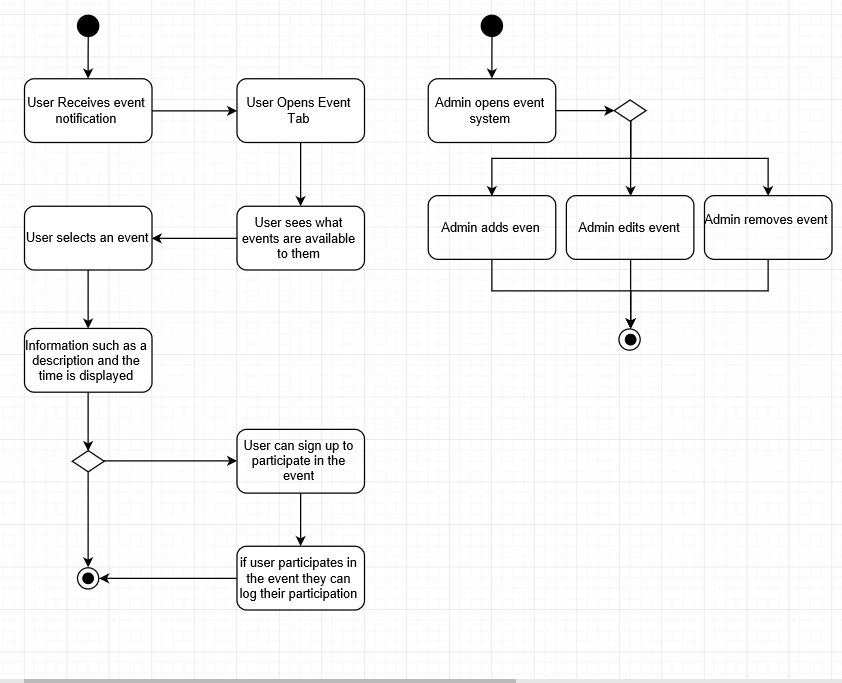
\includegraphics[width=\textwidth]{event/ActivityDiagramTask2.PNG}
		\caption{Events Activity Diagram}
\end{figure}


\subsubsection{Sequence Diagram}
This diagram models time-ordered interaction behaviour between a user logging in and the interaction with the Event subsystem.
\begin{figure}[H]
		\centering
		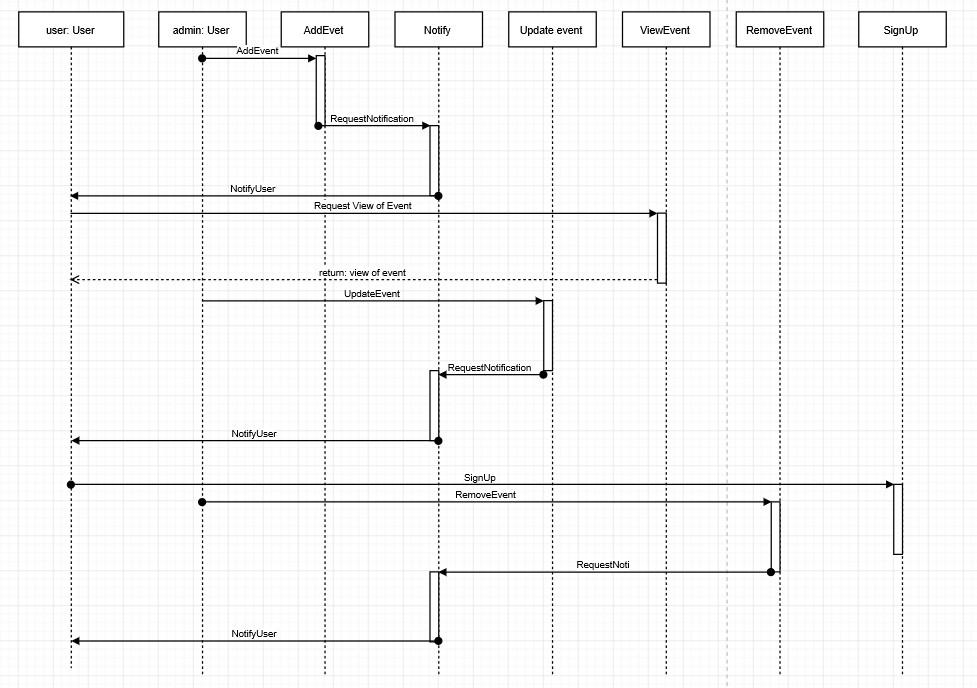
\includegraphics[width=0.7\textwidth]{event/SequenceDiagramTask2.PNG}
		\caption{Events Sequence Diagram}
\end{figure}



\subsubsection{State Diagram}
This diagram models state dependant behaviour of a user with Event Modules.
\begin{figure}[H]
		\centering
		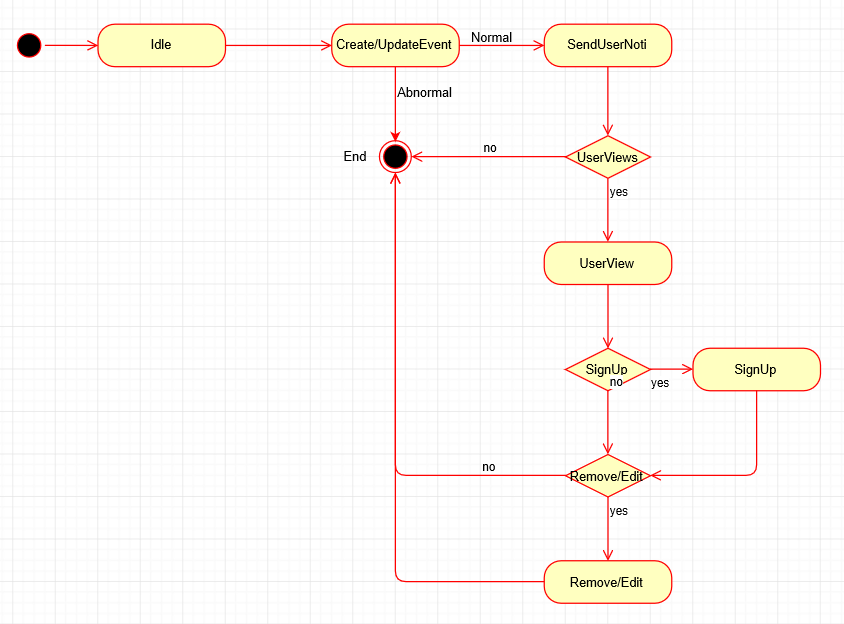
\includegraphics[width=\textwidth]{event/StateDiagramTask2.PNG}
		\caption{Events State Diagram}
\end{figure}




\subsubsection{Use Case Diagram}
Use case diagram which shows the functions of the subsystem as well as relationships of external entities or actors. This refined version also includes a detailed flow of use cases.
\begin{figure}[H]
		\centering
		\includegraphics[width=0.7\textwidth]{event/UserCaseTask2.PNG}
		\caption{Events core functionality }
\end{figure}



	\pagebreak
	\section{Notification Module}
\subsection{Overview}
The notifications module provides notifications to system users regarding particular system updates that a user would like to be notified about through some medium external to the application. 
\subsection{External Interface Requirements}
This section gives a detailed description of the system interfaces, hardware interfaces, software interfaces as well as communication interfaces.
\subsubsection{System Interfaces}
\begin{itemize}
	\item The notification module will interface with any subsystem or module that wishes to send out notifications to users. The subsystem requesting for users to be notified is modelled as the Notifying Module. The Notifying module will interface with the Notification Module through the setState() function to send a notification request. 
	
	\item The notification module will interface with the User module in order to sufficiently dispatch notifications. Each instance of the Notifier class will maintain a list of attached users and will send notifications through the notify() function.
\end{itemize}

\subsubsection{User Interfaces}
\begin{itemize}
	\item The system will dispatch notifications in the form of an \textbf{SMS} to the appropriate users. The SMS will contain the content of the notification and the interface will depend on the user's device.
	
	\item The system will dispatch notifications in the form of an \textbf{email} to the appropriate users. The email will have an appropriate subject and will contain the content of the notification. The interface will depend on the mail application used by the user.
	
	\item The system will dispatch notifications in the form of \textbf{Push Notifications}.  push notifications will contain a title, content and a timestamp. The interface will depend on the user's operating system. 
\end{itemize}

\subsubsection{Hardware Interfaces}
The Notification Module does not have any explicit hardware interfaces

\subsubsection{Software Interfaces}
  \begin{itemize}
  	\item The notification module will communicate with the database in order to get the details of users to be notified.
  \end{itemize}
  
\subsubsection{Communication Interfaces}
	\begin{itemize}
		\item The notification module will need to communicate with an Email API when sending out emails to users
		\item The notification module needs to interface with the SMS Manager API to send SMS's to users.
		\item The notification module will interact with the Operating system push notification service (OSPNS) to allow users to receive push notifications.
	\end{itemize}
	
\subsection{Performance Requirements}
Notifications should be able to perform and guarantee message delivery under high volumes, allow real time notifications to be received and have good network access for this purpose. 

\subsection{Design Constraints}
The notifications must be:
\begin{itemize}
	\item Visually appealing and easy to read, have a gamification point of view
	\item Support viewing on different sizes of device screens
	\item Support colour for all devices
	\item Being able to integrate easily with notification providers
\end{itemize}


\subsection{Software System Attributes}
\subsubsection{Reliability}
The system should make use of a queue to send notifications, so that no messages can get lost on the way and must guarantee that the notification must be delivered.
Notifications should be authentic and be able to verify that delivery of the notification.

\subsubsection{Security}
The sending of the notifications must be secure using proper SMTP setup with SSL encryption for emails, and a authentic SMS provider validated by the WASPA, and a secure means of push notifications using IONIC App that allows secure remote push notifications to all user devices that contain the app.

\subsubsection{Auditability}
All notifications that have been sent by any means, by email, SMS, or even push notifications should be logged on the back-end server.

\subsubsection{Availability}
The notifications module should be available throughout the entire execution of the system since it needs to provide real-time notifications to the user, of events etc. nearby. This becomes vital for the module to be optimised and have good communications network to account for the minimal possible network delay to make meet the real-time expectations.



\subsection{Design}
The Notification Subsystem is designed using 2 design patterns:
\begin{enumerate}
	\item \textbf{Strategy - } This pattern encapsulates the send() function within the Notification class, making it interchangeable. This allows the send() function to vary based on whether the notification is an email notification, SMS notification or a push notification.	
	\item \textbf{Observer - } This pattern defines a one-to-many relationship between the Notifier and User classes so that when the Notifier's state changes, all users are notified automatically.
\end{enumerate}
\newpage
\subsubsection{Class Diagram}
This diagram models the structural elements, their composition and classification.

\begin{figure}[H]
	\centering
	\includegraphics[scale=0.4]{notification/img/ClassDiagram.png}
	\caption{Notification Class Diagram}
\end{figure}

\newpage
\subsubsection{Activity Diagram}
This diagram models work-flow activities and exhibits sequencing, exclusion, synchronization and concurrency.
\begin{figure}[H]
	\centering
	\includegraphics[scale=0.5]{notification/img/activityDiagram.png}
	\caption{Notification Activity Diagram}
\end{figure}


\subsubsection{Sequence Diagram}
This diagram models time-ordered interaction behaviour between the objects within this subsystem.
\begin{figure}[H]
	\centering
	\includegraphics[scale=0.4]{notification/img/SequenceDiagram.png}
	\caption{Notification Sequence}
\end{figure}

\newpage
\subsubsection{State Diagram}
This diagram models state dependant behaviour of an object.
\begin{figure}[H]
	\centering
	\includegraphics[scale=0.5]{notification/img/stateDiagram.png}
	\caption{Notification State Diagram}
\end{figure}




\subsubsection{Use Case Diagram}
This is a refined version of the use case diagram given in the Requirements Specification. It shows the functions of the subsystem as well as relationships of external entities or actors.
\begin{figure}[H]
	\centering
	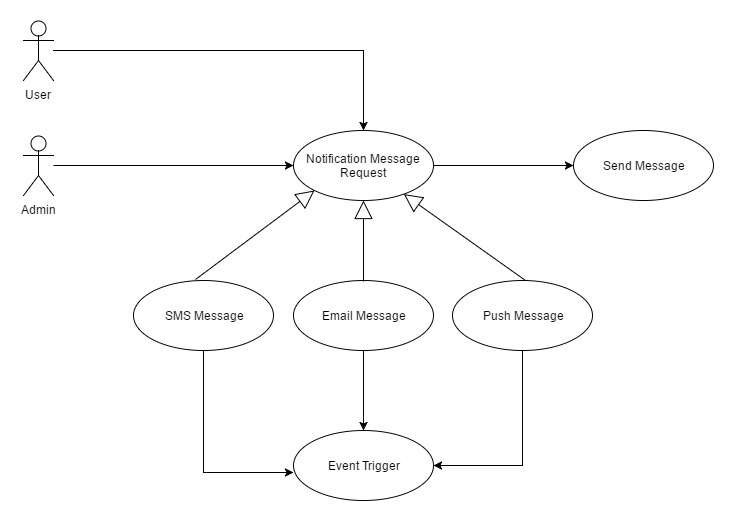
\includegraphics[width=0.7\textwidth]{notification/img/NotificationUseCase.png}
	\caption{Notification core functionality }
\end{figure}

	
\section{Technologies}
The technologies to be used for the system will be discussed below:
\begin{itemize}
	\item TOMCAT - it is a free Apache application server where one can deploy and run JSP and Servlets and provides good logging and management facilities since every app gets wrapped into a war file and is mostly used for web applications as its limited to functionality.
	
	\item WILDFLY - similar to tomcat server but this is a full fledged JavaEE application server for the back-end system.
	
	\item JAVAEE - will be used develop the business logic of NavUP which forms part of the back-end. JavaEE is a good choice for NavUP because this platform uses "containers" to simplify development. JavaEE containers provide for the separation of business logic from resource and lifecycle management, which means that developers can focus on writing business logic, rather than writing enterprise infrastructure. 
	
	\item TCP/IP - 
	
	\item JAX-RS REST - Using the RESTEasy implementation of JAX-RS since it is portable and can run on any Servlet container, and integrates nicely with JBOSS and provides client framework to make writing HTTP clients easy.
	
	\item ACTIVEMQ - 
	
	\item JPA - The Java Persistence API (JPA) is a specification for object-relational mapping in Java. The main advantage JPA will have on NavUP will be its database independence. JPA It provides a database independent abstraction on top of SQL. As long as you're not using any native queries, you don't have to worry about database portability. 
	
	\item POSTGRESQL / POSTGIS - The entire code of the system should be decoupled from which concrete database is used. For NavUP PostgreSQL will be used. It is a mature, efficient and reliable relational database implementation which is available across platforms and for which there is a large and very competent support community
	
	\item JUnit - JUnit will used to perform unit tests on separate modules of NavUP. Junit has been chosen due to its simplicity when testing Java applications. JUnit can be used separately or integrated with build tools like Maven and Ant and third party extensions.
	
	\item JSP - Java Server Pages (JSP) is a technology that helps software developers create dynamically generated web pages based on HTML, XML, or other document types. The main benefit that JSP will have on NavUP is that JSP pages are compiled dynamically into Servlets when requested, so page authors can easily make updates to presentation code.
	
	\item HTML5 \& BOOTSTRAP - The main advantage of using bootstrap on NavUP will be its responsiveness.Creating mobile ready websites is a breeze with Bootstrap thanks to the fluid grid layout that dynamically adjusts to the proper screen resolution. There is virtually no work that needs to be done to achieve proper responsiveness. HTML5 is a markup language used for structuring and presenting content on the internet. One of the coolest things about HTML5 is the new local storage feature which is better than cookies because it allows for storage across multiple windows and also has better security and performance and data will persist even after the browser is closed.
	
	\item JQUERY - 
	
	\item CSS - CSS(Cascading Style Sheet) will be used for styling the web front end of NavUP. It was chosen because of its Lightweight code and because it's easier to maintain and update. 
	
	\item MAVEN - Maven is a powerfull project management tool that is based on POM(project object model).It is used for projects build,dependency and documentation. Maven will be suitable for NavUP because maven projects do not need to store third-party binary libraries in source control, which reduces undue stress on developer checkouts and builds which results in better dependency management
.	
	
	
	\item IONIC v2 - is a open source hybrid mobile application framework which deals with web technologies such as HTML, Angular, JavaScript and Typescript to make a nice looking application with minimal effort, they have their own custom styling to make it easier to build native looking applications with ease. It is also powerful for data processing since v2 works with typescript which is a OOP language derived from JavaScript, this typescript gets transpiled into JavaScript at run time. It unlocks native APIs and features by wrapping Cordova plug-ins into typescript especially good for accessing wireless information and also GPS.
	
	
	
\end{itemize}


	
\end{document}